% =====================================================================
% SkeletonGraph — REFRAMED 2026-07 around the honest finding.
% Maintained by: yashdoke215@gmail.com
% Compile: pdflatex skeletongraph.tex && bibtex skeletongraph && pdflatex skeletongraph.tex
%
% THESIS (do not weaken): high retrieval recall does NOT buy proportional
% cost reduction. It removes the expensive exploration TAIL (p95 -42.5%),
% not the median (+1.9%). pass@1 is a statistical tie (McNemar p=1.0)
% because the benchmark is memorization-saturated (no-retrieval control
% solves 36-44%).
%
% NAMING: internal run tags (claude_v7 / nemotron_v4 / v2) must NEVER
% appear. One result per pipeline, named by what it is. The react-loop arm
% id "fusion" is presented as "SG-Fusion (react)".
%
% \tbd{...} marks numbers pending nemotron_v4 verification completion.
% =====================================================================
\documentclass[11pt,letterpaper]{article}
\usepackage[margin=1in]{geometry}
\usepackage[utf8]{inputenc}
\usepackage{microtype}
\usepackage{booktabs}
\usepackage{graphicx}
\usepackage{xcolor}
\usepackage{hyperref}
\usepackage{amsmath,amssymb}
\usepackage[numbers,sort&compress]{natbib}   % numeric citations: [1], [2,3]
\hypersetup{colorlinks=true,linkcolor=blue!60!black,citecolor=blue!60!black,urlcolor=blue!60!black}
\newcommand{\tbd}[1]{\textcolor{red}{[\textbf{TBD: }#1]}}
\newcommand{\sg}{\textsc{SkeletonGraph}}

\title{High Retrieval Recall Does Not Buy Proportional Cost Reduction:\\
A Controlled Study of Code Retrieval in Frontier Coding Agents}
\author{Yash Doke\\\texttt{yashdoke215@gmail.com}}
\date{\today}

\begin{document}
\maketitle

\begin{abstract}
A growing class of tools promises to make AI coding agents dramatically cheaper
by giving them better code retrieval, with advertised savings ranging from
tenfold to over ninety-nine percent. Those figures are almost always computed the
same way: the tokens a structured query returns are compared against the tokens
it would take to read the relevant files in full. That comparison omits the agent.
It does not tell a practitioner whether more bugs get fixed, or whether the bill
at the end of the month is smaller.

We measure the quantity practitioners actually pay for. Every retrieval pipeline
we test keeps its own interface and is placed in the same harness---the same
model, the same repository tasks, the same edit-and-test loop, with every fix
adjudicated by executing the project's own test suite. We evaluate our system,
\sg{}, which indexes a repository's structure without invoking a language model
and retrieves whole functions rather than files.

Retrieval quality improves substantially. Running inside a production coding agent
over 100 verified tasks, \sg{}'s first search locates the correct file in 83.6\%
of tasks against 66.3\% for the agent's built-in text search, and it identifies
the correct \emph{function} in roughly 80\% of tasks against 0\%---text search returns
files, so naming a function is not something it does poorly but something it
cannot do at all.

The resulting cost saving is real but strongly conditional, and this is our
central finding. On simple tasks \sg{} is slightly \emph{more} expensive, because
its retrieval calls are pure overhead when the agent already knows where to look.
On difficult tasks the saving is large: grouping the same 100 tasks into deciles
by baseline cost, the effect rises monotonically from $+44\%$ on the cheapest
decile to $-42.8\%$ on the most expensive, crossing break-even at roughly \$0.35
per task. Averaged over everything this reads as $-14.6\%$, but the average
conceals the mechanism: the entire saving comes from preventing the agent from
wandering on tasks where it cannot find the code.

We then show this saving has a ceiling that better retrieval cannot lift. Peak
context is unchanged with and without retrieval (44.1k versus 44.9k tokens):
retrieval does not shrink the agent's working set, it shortens the path to it, so
cost falls only in proportion to steps saved ($-21.4\%$ steps, $-23.6\%$ tokens).
An agent acquires whatever the task requires---from the retriever if supplied, by
itself otherwise---and whatever it acquires early is re-sent on every later step.
We test this four ways, giving the agent more context, less context, removing its
need to re-read, and forcing it to verify; all four degraded cost or correctness.
A fifth test, routing each task to whichever system would be cheaper, shows even a
perfect oracle gains only 14\% and does so by selecting runs that failed early.

The practical claim is therefore precise: structural retrieval cuts the cost of
expensive tasks by roughly 40\% while leaving ordinary ones alone, and beyond that
point cost is governed by how the model implements and validates rather than by
how well it searches. Harness, task lists, and per-task records are released so
this can be checked rather than believed.
\end{abstract}

\section{Introduction}

An AI coding agent solving a real repository issue spends its budget in three
places: finding the code to change, writing the change, and running tests until
they pass. Tools that improve the first of these are now a small industry, and
they advertise large savings---commonly an order of magnitude, sometimes over
99\%. Almost all of those figures come from the same calculation: count the tokens
a structured query returns, count the tokens it would take to read the
corresponding files end to end, and report the ratio.

That calculation leaves out the agent, and the omission matters more than it
appears. An agent does not read whole files by default, so the denominator
describes a workflow nobody runs. It does not stop once it has found the code, so
the numerator covers a fraction of the trajectory. And it is not billed per
retrieved token: it is billed for the entire conversation, re-sent on every step.
A retrieval improvement is therefore a claim about one phase of a three-phase
process, reported in units nobody is charged in.

This paper asks what better retrieval is actually worth once the agent is put
back in. We compare retrieval strategies inside a single harness that holds
everything else fixed---the same model, the same repository tasks, the same
edit-and-submit interface---and we do not accept a system's own judgment of
whether it solved a task: every candidate patch is applied and the project's real
test suite is executed in a container.

Throughout, we compare against what we call the agent's \emph{built-in tools}:
the text search, file glob, and file read that a production coding agent ships
with and is heavily trained to use. This is a deliberately strong baseline. Much
of the published work in this area compares a retrieval system against reading
entire files, which no competent agent does; a retrieval layer that only beats an
artificially weakened baseline has not been evaluated.

\paragraph{What we find.}
Structural retrieval works. On its first search, built-in text search recovers
66.3\% of the files a task requires and can never name the function to
change---text search matches lines and returns files, so function-level retrieval
is not something it does badly, it is something it cannot do. Our system recovers
83.6\% of the files on its first search and identifies the correct function in
roughly 80\% of tasks. Against seven alternative strategies it consumes the fewest
tokens by a wide margin.

And yet the money moves much less than that suggests, and not where one would
expect. Deployed inside a production agent over 100 tasks, retrieval makes simple
tasks slightly \emph{more} expensive and removes roughly 40\% of the cost of the
hardest ones, crossing break-even around \$0.35 per task. Solve rate does not
change at all.

The explanation turns out to be simple, and is visible in a single measurement:
the peak context the agent accumulates is the same with retrieval as without it
(44.1k versus 44.9k tokens). Retrieval does not shrink what the agent carries; it
shortens the path to the answer. Cost falls in proportion to the steps saved and
no further. Underneath that is a fact about how agents consume context: an agent
acquires whatever the task requires, from us if we supply it and by itself if we
do not, and anything acquired early is re-sent on every step that follows. Give
it less and it fetches the difference itself, adding steps; give it more and the
surplus is charged repeatedly. Until the agent's own step count falls, the bill
keeps growing regardless of retrieval quality.

\paragraph{Contributions.}
\begin{enumerate}
\item \textbf{A decoupling result.} We show that large gains in retrieval accuracy
do not produce proportional cost reduction in a deployed agent, and we quantify
the gap: unchanged median cost against a 42.5\% reduction at the 95th percentile
(Section~\ref{sec:decoupling}).

\item \textbf{An explanation, not just an observation.} We give a cost model for
agentic retrieval, show that the context an agent carries is bounded below by
what the task requires, and derive why payload shaping has limited leverage in
both directions while step count does not (Sections~\ref{sec:model}
and~\ref{sec:floor}).

\item \textbf{Evidence that the benchmark cannot see retrieval.} A control that
receives no repository code at all solves 36--44\% of tasks on the standard
benchmark. Retrieval quality is not measurable through solve rate here---which
also invalidates solve-rate comparisons that would favor us
(Section~\ref{sec:saturation}).

\item \textbf{Four negative results with diagnostic value.} We attempt to convert
retrieval quality into savings four ways and report all four failures, including
one where removing a genuinely wasteful step made outcomes worse because the
waste was load-bearing (Section~\ref{sec:interventions}).

\item \textbf{A reproducible artifact.} The harness, the frozen task lists, and
per-task records are released, along with an index that any user can rebuild from
source because building it never calls a language model.
\end{enumerate}

\section{Background: What a Code-Context System Is For}
\label{sec:background}

\subsection{The task and where its cost comes from}
A repository-scale coding agent is given an issue and repository access, and must
produce a patch that passes hidden tests. Its trajectory has three phases that
consume budget very differently:

\begin{enumerate}
\item \textbf{Localization} --- find the code to change. Cost scales with how
much of the repository the agent must inspect before it is confident.
\item \textbf{Implementation} --- write the edit. Cost scales with how much code
must be understood well enough to modify correctly.
\item \textbf{Validation} --- run tests, read failures, repair. Cost scales with
how many repair iterations are needed, and is unbounded in the worst case.
\end{enumerate}

A retrieval layer can only act directly on phase 1. This is obvious once stated,
but the prevailing evaluation practice obscures it: reporting retrieval token
savings in isolation implicitly assumes phase 1 dominates. A central goal of this
paper is to measure how much of the budget phase 1 actually is.

\subsection{The design space, and what each design optimizes}
\label{sec:designspace}
Existing systems are not arbitrary---each embodies a hypothesis about which term
in the cost dominates. Making those hypotheses explicit predicts each system's
cost profile before any measurement.

\paragraph{Prompt injection (repository maps).}
Aider \citep{aider} builds a PageRank-ranked skeleton of the repository and
injects it into the prompt. \emph{Hypothesis:} the agent's problem is not knowing
what exists, so give it a map up front. \emph{Implied cost:} the map is part of
the fixed prompt and is therefore re-sent every turn --- a one-time modelling
decision billed $T$ times. Our measurements confirm this is the most expensive
strategy tested by a wide margin.

\paragraph{Graph query (knowledge-graph servers).}
Codebase-Memory \citep{cbmem} and Graphify \citep{graphify} extract an entity
graph, usually with an LLM pass per repository, and expose queries over it.
\emph{Hypothesis:} the agent's problem is navigating relationships, so answer
relationship queries on demand. \emph{Implied cost:} pay-per-query rather than
up-front, but query results are entity-shaped rather than edit-shaped, so
payloads tend to be broad. There is also a hidden cost these systems' headline
numbers exclude: graph construction requires an LLM pass over every repository.

\paragraph{Lexical search (grep, BM25).}
\emph{Hypothesis:} identifiers are highly discriminative in code, so text search
is sufficient. This is a stronger baseline than it appears; \citet{agentless}
show that a simple hierarchical localize-repair pipeline is competitive with
elaborate agentic scaffolding, and our own results show lexical navigation
reaching the gold file in the large majority of tasks. \emph{Implied cost:} cheap
per call, but file-granular --- the agent must read to narrow further, and those
reads are the dominant token sink we measure.

\paragraph{Structural retrieval (this work).}
\emph{Hypothesis:} the unit an agent edits is a \emph{function}, so retrieval
should return functions, ranked by combined lexical, semantic and structural
evidence. This is supported independently: \citet{granularity} find function-level
localization yields the highest repair rate against both line-level and file-level
granularity, while noting the optimum is task-dependent; and \citet{locagent} show
graph-guided localization reaching high file-level accuracy at reduced cost.
\emph{Implied cost:} pay-per-query with edit-shaped payloads. Our contribution is
to measure what that buys end-to-end, and to report honestly that it buys less
than the design predicts.

\subsection{What the literature already suggests about the ceiling}
Two prior findings anticipate our result without stating it in cost terms.
\citet{coderagbench} evaluate retrieval-augmented code generation broadly and
report that although high-quality context improves generation, retrievers
struggle to fetch useful context \emph{and generators fail to exploit additional
context effectively}. \citet{granularity} similarly find diminishing and
task-dependent returns as localization granularity sharpens. Both point to the
same place: the bottleneck migrates out of retrieval. Our contribution is to
measure that migration in dollars and turns inside a real agent loop, and to
explain it with a cost model.

\section{Related Work}

\paragraph{Agentic software engineering.}
SWE-agent \citep{sweagent} introduced agent-computer interfaces for repository
tasks; OpenHands \citep{openhands} generalized the platform.
\citet{agentless} argued the opposite direction---that much agentic
machinery is unnecessary---with a three-phase localize/repair/validate pipeline
competitive with agent scaffolds at low cost. We inherit that scepticism: our
baseline is a strong native-tools agent, not a weakened one, because a retrieval
layer that only beats a hobbled baseline has not been evaluated.

\paragraph{Localization as a first-class problem.}
LocAgent \citep{locagent} parses repositories into heterogeneous graphs for
multi-hop localization, reaching up to 92.7\% file-level accuracy with a
fine-tuned 32B model at roughly 86\% cost reduction relative to proprietary
models. \citet{granularity} isolate granularity itself and find function-level
best on average but task-dependent. Our function-level results
(Figure~\ref{fig:retrieval}) are consistent with both. Where we differ is the
dependent variable: these works measure localization accuracy, while we measure
what accuracy converts into once an agent must also implement and validate.

\paragraph{Retrieval-augmented code generation.}
CodeRAG-Bench \citep{coderagbench} is the closest methodological precedent---a
holistic benchmark separating retrieval quality from end-to-end generation. Their
finding that generators under-exploit retrieved context is, in our framing, the
generation-side counterpart of the cost-side ceiling we measure.

\paragraph{Code-context products.}
Codebase-Memory \citep{cbmem}, Graphify \citep{graphify}, and Aider's repository
map \citep{aider} are the deployed systems in this category. They differ from
this work in evaluation rather than ambition: headline numbers are token-count
comparisons against whole-file reading, self-graded, or measured without an
agentic loop. Where an agentic evaluation is reported, a quality cost accompanies
the saving---one such report describes roughly $10\times$ fewer tokens at 90\% of
baseline answer quality. Our result differs in kind: a smaller cost reduction
with \emph{no} measurable quality loss, and paired per-task records that make the
comparison checkable.

\paragraph{Memory and context management.}
MemGPT \citep{memgpt} treats context as a paging problem; HierMem
\citep{hiermem} organizes agent memory hierarchically. \sg{} is deliberately
narrower---a structural index and reranker, not a memory manager---and zero-LLM
at index time, so index construction is never billed to a model.

\paragraph{Benchmarks and contamination.}
SWE-bench \citep{swebench} is the standard benchmark; its contamination is now
widely discussed and major evaluators have moved away from reporting SWE-bench
Verified as a headline. Decontaminated successors such as SWE-rebench
\citep{swerebench} draw continuously from thousands of repositories with tasks
postdating model cutoffs. Our no-retrieval control quantifies the contamination
effect directly in our own setting (Section~\ref{sec:saturation}).

\section{Method}

\subsection{Design principle: a systems comparison, not a tool ablation}
Each pipeline keeps its native retrieval interface. Baselines (\texttt{grep},
\texttt{bm25}, \texttt{hybrid}) receive the harness's standard tool set;
competitor systems receive their own tools (graph query, snippet fetch, repo-map
injection); \sg{} receives its own search and expand tools. What is held
constant is the substrate: model, task set, edit/submit interface, turn budget,
and verification. This measures \emph{deployed systems}, the unit practitioners
actually choose between, rather than a retrieval function in isolation.

\subsection{\sg{}}
\sg{} builds a zero-LLM structural index with tree-sitter \citep{treesitter}
parsers, producing a symbol table of fully-qualified names with line ranges,
signatures, docstrings, and a call graph. Retrieval fuses three ranked lists by
reciprocal rank fusion \citep{rrf}: BM25 \citep{bm25} (lexical), a dense code
embedding model (semantic), and a structural reranker over the symbol graph.
Fusion is used rather than a tuned linear combination deliberately---RRF has no
score-scale parameters to fit, so no part of the ranking is tuned on the
evaluation set.

Because indexing invokes no language model, index construction is not billed to a
model and can be rebuilt by any user from source. This is a substantive
difference from the graph-building systems in Section~\ref{sec:designspace},
whose extraction step requires an LLM pass over every repository---a per-repo
cost their reported token savings exclude, and one that must be re-paid whenever
the repository changes materially.

The retrieval surface is exposed to agents over the Model Context Protocol
\citep{mcp}, which is what makes the deployment measurement in
Section~\ref{sec:decoupling} possible against an agent we do not control.

We evaluate two operating points. \emph{SG-Fusion} is the three-way fusion
above. \emph{SG-Rerank} drops the dense leg (a BM25 recall pool reordered by
structural confirmation), requiring no embedding model or prewarm.

\subsection{Harnesses}
\textbf{React loop.} Our own agent loop offers tools directly to the model, with
no MCP handshake. This is the axis on which competitor systems can be compared
fairly (Section~\ref{sec:exclusion} explains why they cannot be compared inside
a headless frontier agent).

\textbf{Frontier-agent deployment.} \sg{} runs as a real MCP server driven by a
frontier coding agent in headless mode, against an unmodified native-tools
baseline. This measures deployment economics under an agent we do not control.

The two harnesses implement the same three-way fusion algorithm in separate code
paths; we present them as SG-Fusion (react) and SG-Fusion (MCP) and never pool
their numbers.

\subsection{A cost model for agentic retrieval}
\label{sec:model}
Before measuring, it is worth writing down what an agent is actually billed for,
because the discrepancy between that quantity and the quantity competitors report
is the origin of the whole result.

Let a trajectory consist of turns $t = 1 \dots T$. At each turn the model is sent
the entire accumulated conversation. Write $c_t$ for the context size at turn $t$.
Billed input tokens are then
\begin{equation}
N \;=\; \sum_{t=1}^{T} c_t \;=\; \sum_{t=1}^{T}\Big( c_0 + \textstyle\sum_{s<t} r_s + \sum_{s<t} a_s \Big),
\label{eq:cost}
\end{equation}
where $c_0$ is the fixed prompt overhead, $r_s$ the tokens returned by the tool
called at turn $s$, and $a_s$ the model's own output at turn $s$. Two consequences
follow immediately, and both are borne out empirically.

\paragraph{Tool output is charged once per remaining turn, not once.}
A result $r_s$ appears in every subsequent context, so its true cost is
$r_s\,(T-s+1)$. Retrieved tokens are therefore \emph{not} interchangeable with
saved read-tokens: an early, large payload is the most expensive object in a
trajectory. We use this weighting for attribution in Section~\ref{sec:analysis}.

\paragraph{Reducing $r$ alone cannot reduce $N$ much.}
Competitor claims optimize $\sum_s r_s$: the token cost of retrieval versus
reading whole files. But in Equation~\eqref{eq:cost} that term is one of three,
and it is not the dominant one once $c_0$ and the accumulated $a_s$ are included.
Writing $\bar{c}$ for mean context size, $N \approx T\bar{c}$, so
\begin{equation}
\frac{\Delta N}{N} \;\approx\; \frac{\Delta T}{T} \;+\; \frac{\Delta \bar{c}}{\bar{c}}.
\label{eq:decomp}
\end{equation}
A retrieval layer can act on either term: it can shorten the trajectory (fewer
turns to localize) or slim the context (less material carried). Our central
empirical finding, Section~\ref{sec:decoupling}, is that structural retrieval
moves the first term and leaves the second at approximately zero---which bounds
the achievable saving at the turn reduction, independent of how good retrieval
gets. This is a structural ceiling, not a tuning failure, and it predicts the
observed $-21\%$ turns / $-24\%$ tokens correspondence before we measure it.

\paragraph{Why the median and the mean must be reported separately.}
Equation~\eqref{eq:cost} is quadratic in $T$ when a trajectory wanders: extra
turns both add their own context and re-send everything prior. Task cost is
therefore heavy-tailed, and a mean over tasks is dominated by its upper tail. A
retrieval layer that truncates long trajectories will move the mean substantially
while leaving the median untouched. Reporting only a mean---as the aggregate
percentages in this literature do---cannot distinguish "everything got cheaper"
from "the disasters stopped," which are very different products.

\subsection{The irreducible context floor}
\label{sec:floor}
Equation~\eqref{eq:decomp} leaves open how far $\bar{c}$ can be pushed down. We
argue it is bounded below, and that the bound is set by the model's task rather
than by the retrieval system's cleverness.

An agent must acquire enough material to write a correct edit. Call that quantity
$c^{*}$: the minimum context sufficient for the task. A retrieval layer chooses
what to hand over, but it does not choose $c^{*}$ --- that is a property of the
bug and of what the model needs to see to be right. Two regimes follow:

\begin{itemize}
\item If the layer returns \emph{less} than $c^{*}$, the agent does not fail
quietly: it goes and gets the difference itself, with its own tools. The tokens
reappear as reads and greps, and the extra retrieval turns are added on top. Cost
is relocated, not saved.
\item If it returns \emph{more} than $c^{*}$, the surplus is not merely wasted
once. By Equation~\eqref{eq:cost} it is re-sent on every remaining turn, and the
surplus is delivered \emph{early} --- so it carries the largest possible
multiplier.
\end{itemize}

This is the sharpest practical consequence of the model, and it explains a result
that surprised us. A payload delivered at turn 1 is billed roughly $T$ times. An
agent behaves exactly as designed: it consumes what it is given, and everything it
consumes early persists in context for the rest of the trajectory. Consequently,
\textbf{shaping the payload has bounded leverage in both directions} --- below
$c^{*}$ the agent recovers the shortfall itself, and above $c^{*}$ the surplus is
amortized against the agent rather than against the retrieval layer. The only term
with unbounded leverage is $T$.

And $T$ is not a retrieval variable. After localization, turn count is governed by
implementation and validation: how many edits the model attempts, whether it runs
tests, how it reacts to a failure. A retrieval layer influences $T$ only through
the localization prefix. Once that prefix is short, further retrieval improvement
acts on a term that has already gone to zero.

Section~\ref{sec:interventions} reports three attempts to beat this bound --- one
below $c^{*}$, one at it, one attempting to control $T$ directly --- and the
failure mode of each is the one this section predicts.

\subsection{Metrics and statistics}
We report Docker-verified pass@1; per-task cost, turns, and total input tokens;
peak context; file- and function-level retrieval hit rate; first-search
precision; and per-tool call counts. Cost is imputed from token counts under one
provider's published pricing, applied identically to every arm.

Following Section~\ref{sec:model} we report the full cost distribution
(p50/p75/p90/p95), not only means. Paired comparisons use McNemar's exact test
for pass@1 and a paired bootstrap ($10^4$ resamples of task \emph{pairs}) for
cost and turn deltas. We resample pairs and recompute the aggregate ratio rather
than averaging per-task percentage changes, because the mean of per-task ratios
diverges from the ratio of means when some tasks are near-zero cost---a
difference large enough in our data to flip the sign of the reported effect.

\section{Results}

\subsection{Retrieval quality: what each approach can and cannot find}
The first question is whether structural retrieval finds the code better than the
text search an agent already has. It does, and Figure~\ref{fig:retrieval} shows
the result has two distinct parts that are easy to conflate.

\begin{table}[t]
\centering
\begin{tabular}{lrr}
\toprule
& Built-in tools & + \sg{} \\
\midrule
Correct file found by the \emph{first} search & 66.3\% & \textbf{83.6\%} \\
Correct file found \emph{eventually} (any search) & 83.4\% & 90.7\% \\
Correct \emph{function} identified & 0\% & \textbf{79--81\%} \\
\midrule
Precision of the first search & 61.8\% & 34.2\% \\
\bottomrule
\end{tabular}
\caption{Retrieval accuracy inside the production agent, 100 tasks. File rows are
\emph{recall}---the fraction of a task's gold files returned, averaged over
tasks---not the weaker ``at least one file matched''. The first two rows differ in
an important way: both approaches usually reach the right file \emph{eventually},
but the built-in tools get there by reading whereas \sg{} returns it immediately,
and the gap between 66.3\% and 83.4\% for the baseline is what that hunting costs.
The function row is given as a range because gold function names recovered from
patch hunks are approximate: 81\% against the released gold set, 79\% after a
stricter disambiguation pass. Both are reported; neither changes any conclusion.}
\label{tab:retrieval}
\end{table}

At the level of \emph{which file to edit}, both approaches work, and the gap
depends on when you measure. On its first search \sg{} finds the right file 83.6\%
of the time against 66.3\% for text search---but given the whole trajectory, the
baseline eventually reaches it 83.4\% of the time. Text search is a genuinely
strong baseline, consistent with prior work finding simple pipelines competitive
with elaborate scaffolding \citep{agentless}. The difference is not whether it
arrives but how much it spends arriving, and Section~\ref{sec:analysis} shows
those intervening reads are the single largest token consumer in the baseline.

At the level of \emph{where in the file to edit}, the gap is not one of degree.
\sg{} names the correct function in about 80\% of tasks; text search names it in zero.
This is not a tuning deficit: text search matches lines and reports the files
containing them, so a function is not an object it can return. That function-level
granularity is the right target is supported independently---\citet{granularity}
find function-level localization produces higher repair rates than either
file-level or line-level.

This accuracy is not free, and the price is paid in precision, which runs the
other way: 34.2\% for \sg{} against 61.8\% for built-in search. Read plainly,
\sg{} much more reliably includes the right code and also includes more code that
turns out not to be needed. It finds the right neighbourhood and hands over the
neighbourhood. Section~\ref{sec:scope} shows this is exactly the mechanism behind
its worst individual cases---the trade a structural retriever makes is breadth in
exchange for reliably covering the target.

\begin{figure}[t]
\centering
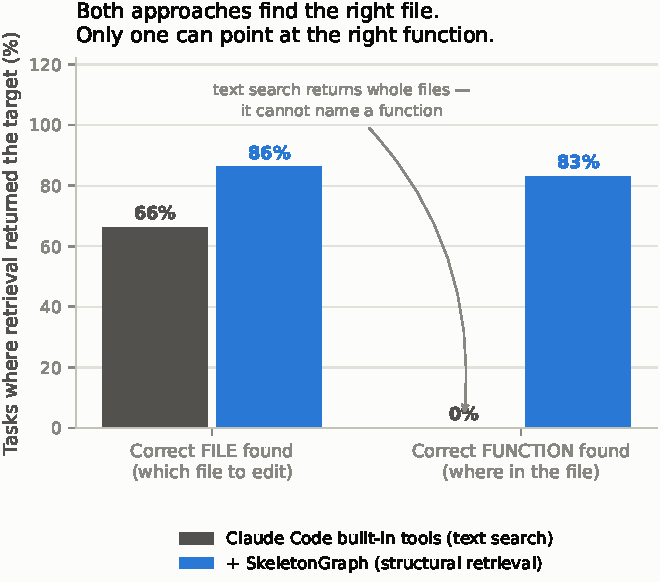
\includegraphics[width=0.72\linewidth]{figures/fig_retrieval.pdf}
\caption{Retrieval accuracy at two granularities (frontier agent, 100 tasks).
The function-level gap is not a tuning difference: lexical search returns file
matches, so its function-level rate is $0\%$ by construction. This is the
largest quality difference we measure anywhere---and
Section~\ref{sec:decoupling} shows it does not transfer to cost.}
\label{fig:retrieval}
\end{figure}

\subsection{The decoupling: retrieval improves, the typical bill does not}
\label{sec:decoupling}
Given that retrieval accuracy improves as much as it does, the natural
expectation is that cost falls correspondingly. It does not, and the shape of
what happens instead is the paper's central result.

The headline average is a 14.6\% cost reduction across 100 paired tasks. That
average is misleading on its own, in a specific and instructive way: \sg{} is
cheaper on only 40 of the 100 tasks, and the cost of the median task rises very
slightly ($+1.9\%$). Nearly the entire average saving comes from a small number
of expensive tasks. Table~\ref{tab:tail} shows the distribution.

\begin{table}[t]
\centering
\begin{tabular}{lrrr}
\toprule
& \multicolumn{2}{c}{Cost per task (USD)} & \\
\cmidrule(lr){2-3}
Task cost percentile & Built-in tools & + \sg{} & Change \\
\midrule
50th (the median task) & \$0.255 & \$0.260 & $+1.9\%$ \\
75th                   & \$0.581 & \$0.489 & $-15.8\%$ \\
90th                   & \$1.010 & \$0.752 & $-25.6\%$ \\
95th (the worst tasks) & \$1.559 & \$0.896 & $-42.5\%$ \\
\midrule
Average across all tasks & \$0.434 & \$0.371 & $-14.6\%$ \\
\bottomrule
\end{tabular}
\caption{Where the saving lives. Each row is a point in the cost distribution
over the same 100 tasks: the 50th-percentile row is the typical task, the
95th-percentile row is among the most expensive. Retrieval does nothing for the
typical task and removes over 40\% of the cost of the worst ones. The average in
the final row is produced by the bottom rows, not spread across them. Paired
bootstrap 95\% confidence interval on the average change:
$[-25.3\%, -1.2\%]$.}
\label{tab:tail}
\end{table}

\paragraph{The effect is monotone in task difficulty, and it crosses zero.}
Table~\ref{tab:decile} groups the same 100 tasks into deciles by what the baseline
spent. The trend is close to perfectly ordered, and it shows something the summary
statistics hide: on easy tasks \sg{} is not merely neutral, it is
\emph{consistently more expensive}.

\begin{table}[t]
\centering
\begin{tabular}{clrr}
\toprule
Decile & Baseline cost range & Cost change & Tasks where \sg{} was cheaper \\
\midrule
1  & \$0.10 -- \$0.12 & $+44.0\%$ & 0 / 10 \\
2  & \$0.12 -- \$0.14 & $+55.1\%$ & 0 / 10 \\
3  & \$0.14 -- \$0.16 & $+22.0\%$ & 0 / 10 \\
4  & \$0.16 -- \$0.18 & $+18.0\%$ & 2 / 10 \\
5  & \$0.19 -- \$0.25 & $+95.3\%$ & 2 / 10 \\
6  & \$0.26 -- \$0.31 & $+18.7\%$ & 4 / 10 \\
\midrule
7  & \$0.31 -- \$0.41 & $-10.5\%$ & 7 / 10 \\
8  & \$0.43 -- \$0.67 & $-25.9\%$ & 8 / 10 \\
9  & \$0.68 -- \$0.96 & $-28.0\%$ & 8 / 10 \\
10 & \$1.01 -- \$2.12 & $\mathbf{-42.8\%}$ & 9 / 10 \\
\bottomrule
\end{tabular}
\caption{The crossover. Tasks grouped into deciles by baseline cost. Retrieval
costs money on the six cheapest deciles and saves money on the four most
expensive, with break-even near \$0.35 per task. The rightmost column is nearly
perfectly ordered (0,0,0,2,2,4,7,8,8,9), which is what distinguishes this from
noise. Decile~5 contains one volatile outlier that inflates its percentage; its
win count is consistent with its neighbours.}
\label{tab:decile}
\end{table}

Two things follow. First, there is a \textbf{break-even complexity} at roughly
\$0.35 per task: below it retrieval is overhead, above it retrieval pays, and the
return grows with difficulty. Second, the ordering of the win-count column
(0,0,0,2,2,4,7,8,8,9) is what makes this a law rather than an artifact---a noisy
effect would not order itself that cleanly across ten independent groups.

The mechanism is straightforward once stated. \sg{} adds a fixed overhead: its own
retrieval calls, which are billed whether or not they were needed. On a \$0.11
task that overhead is a large fraction of the total. On a \$2.00 task it is
negligible, and what dominates instead is whether the agent found the code without
a prolonged hunt. Restricting to tasks where the baseline spent at least \$1.00,
the saving is 42.8\%; above \$1.50, 45.0\%. Turn count falls 21.4\% overall
(95\% CI $[-30.0\%, -10.5\%]$) and total tokens 23.6\%.

Figure~\ref{fig:tail} makes the shape visible by ordering tasks from cheapest to
most expensive: the two cost curves lie on top of each other for roughly the first
two thirds of tasks and separate only at the end. Figure~\ref{fig:scatter} shows
the same 100 tasks individually against a line of equal cost.

\paragraph{Why the expensive tasks are where the saving is.}
The mechanism is not that retrieval works better on hard tasks. It is that
expensive tasks are expensive \emph{because the agent could not find the code},
and that is the one failure retrieval prevents. When the baseline localizes
quickly, its trajectory is short and there is nothing to save; \sg{} adds its own
retrieval calls and comes out marginally behind, which is the $+1.9\%$ at the
median. When the baseline cannot localize, it searches, reads, searches again,
and each of those steps re-sends everything accumulated so far---the quadratic
behaviour of Equation~\eqref{eq:cost}. Those are the runs that reach \$1.50 and
beyond, and they are exactly the runs where handing the agent the right function
immediately collapses the trajectory. A concrete instance appears in
Section~\ref{sec:scope}: a task on which the baseline spent 50 turns and \$1.84
exploring, and \sg{} finished in 14 turns and \$0.43.

A practitioner reading only the $-14.6\%$ average would reasonably expect their
bill to fall by about a seventh across the board. The correct expectation is that
most tasks cost the same and the occasional runaway task stops running away.

\begin{figure}[t]
\centering
\begin{minipage}[t]{0.52\linewidth}
\centering
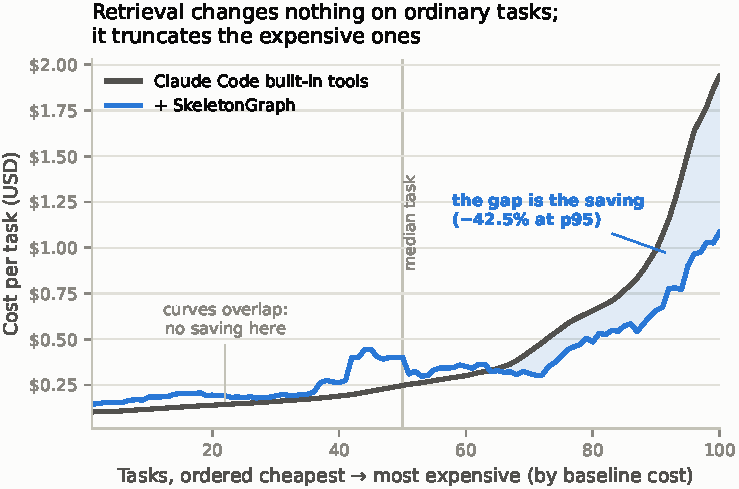
\includegraphics[width=\linewidth]{figures/fig_tail.pdf}
\end{minipage}\hfill
\begin{minipage}[t]{0.44\linewidth}
\centering
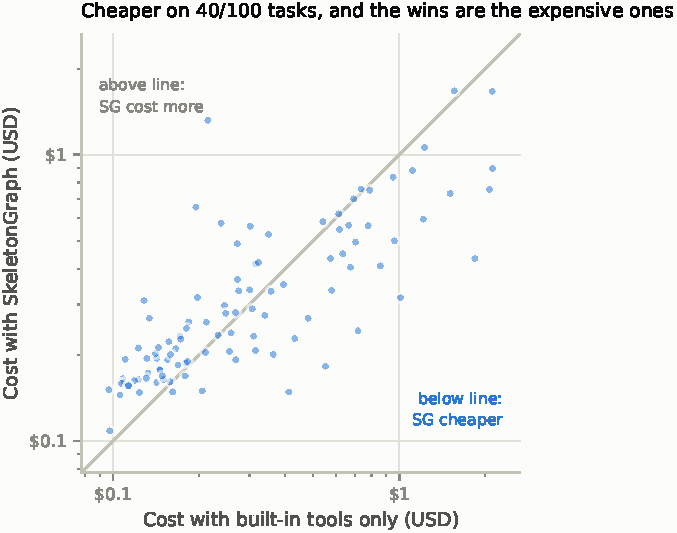
\includegraphics[width=\linewidth]{figures/fig_paired_scatter.pdf}
\end{minipage}
\caption{\textbf{Left:} cost by percentile. The shaded region is the saving; it
opens only above the median. \textbf{Right:} the same 100 tasks, paired. Points
below the line are tasks where \sg{} was cheaper. Both panels are the same
finding at different resolutions.}
\label{fig:tail}
\label{fig:scatter}
\end{figure}

\paragraph{The measurement that explains the ceiling.}
Section~\ref{sec:model} decomposed cost into how many steps the agent takes and
how much context it carries per step. We can now say which of the two retrieval
actually moves, and the answer is unambiguous. The peak context the agent
accumulates is 44{,}129 tokens with built-in tools and 44{,}892 with \sg{}: the
same, to within 2\%.

This is worth stating in plain terms, because it is the paper's explanatory
centre. \emph{Retrieval does not give the agent a smaller working set.} The agent
ends up holding just as much material either way. What changes is how quickly it
assembles that material---21.4\% fewer steps---and cost falls by almost exactly
that proportion, 23.6\%. The two numbers matching is not a coincidence; it is the
identity in Equation~\eqref{eq:decomp} with one of its two terms measured at zero.

The consequence is a ceiling that no amount of retrieval quality can lift. If the
context term does not move, then cost reduction cannot exceed step reduction, and
step reduction is bounded by how much of the trajectory was spent searching in the
first place. Once localization is fast, the remaining steps belong to writing the
fix and running the tests, and a retrieval layer has no purchase on either.

\subsection{Solve rate is a tie, and the benchmark explains why}
\label{sec:saturation}
Solve rate is statistically indistinguishable: 75/100 for \sg{} versus 74/100
native, with 68 shared solves, 7 \sg{}-only and 6 native-only (McNemar exact,
$p=1.0$). We do not claim a solve-rate improvement.

The reason is benchmark saturation. In the react loop, a \texttt{none} control
receiving \emph{no repository code at all} solves 36--44\% of tasks, against
42--45\% for the best retrieval arm. Retrieval is worth a few points at most
here, because the tasks are drawn from twelve heavily-studied open-source
repositories the model has substantially memorized. Any solve-rate comparison
between retrieval systems on SWE-bench Verified is therefore measuring
memorization plus noise, not retrieval.

\subsection{A systems comparison on a second model family}
\label{sec:systems}
The deployment result compares \sg{} against the agent's built-in tools. To compare against
\emph{other retrieval systems} we use the react loop, where every pipeline is
offered its own tools directly and no MCP handshake can exclude a competitor
(Section~\ref{sec:exclusion}). Figure~\ref{fig:tokens} places each system on the
two axes that matter jointly.

\begin{figure}[t]
\centering
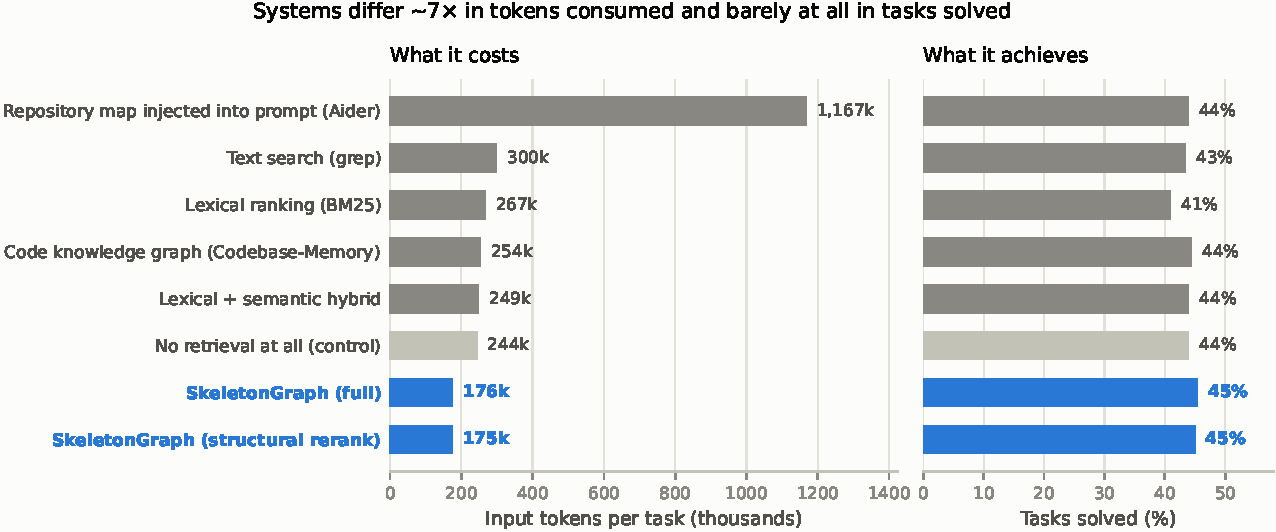
\includegraphics[width=0.82\linewidth]{figures/fig_token_efficiency.pdf}
\caption{Whole systems on a second model family (120B-class open model, 100
SWE-bench Verified tasks; each pipeline keeps its own retrieval interface). The
horizontal spread is an order of magnitude; the vertical spread is a few points
and is not statistically significant. Note the position of the no-retrieval
control.}
\label{fig:tokens}
\end{figure}

Three things in this figure are worth stating explicitly.

\paragraph{The vertical axis is nearly flat, including for the control.}
Solve rates span roughly 41--45\% across every system tested, and the
\texttt{none} arm---which receives no repository code at all---sits at 44\%,
within noise of the best retrieval pipeline. On this benchmark, retrieval is
worth about one point of solve rate. We regard this as the single most important
methodological fact in the area, and return to it below.

\paragraph{The horizontal axis is not flat at all.}
Systems differ by roughly $7\times$ in tokens consumed to reach the same
outcome. Aider's repository map is the clearest case: injecting a PageRank-ranked
skeleton into the prompt costs $\sim$1.17M input tokens per task against
\sg{}'s $\sim$176k. Equation~\eqref{eq:cost} explains why---an injected map is
part of $c_0$ and is therefore re-sent on \emph{every} turn, so a one-time
"context" decision is billed $T$ times. Graph-query systems
(Codebase-Memory, $\sim$254k) sit between the two: they fetch on demand rather
than injecting, but return broader payloads than a function-level fetch.

\paragraph{Retrieval quality and token cost are separately optimizable.}
\sg{}'s two operating points make this concrete. SG-Rerank achieves the best
function-level recall of any arm (0.404 versus 0.342 for BM25 and 0.228 for the
graph-query competitor) at the lowest token cost of any arm---while its solve
rate is indistinguishable from a system using $6\times$ the tokens. Retrieval
quality is real and measurable; it simply is not what determines whether the
task is solved on this benchmark.

\begin{table}[t]
\centering
\begin{tabular}{lrrrrr}
\toprule
Retrieval backend & $n$ & pass@1 & rec@1 & funcHit & Cost \\
\midrule
\sg{}-Fusion            & 100 & \textbf{42.0\%} & 0.737 & \textbf{57\%} & \textbf{\$0.052} \\
BM25                    & 100 & 41.0\% & 0.642 & 43\% & \$0.074 \\
Graph-query competitor  & 100 & 41.0\% & 0.223 & 9\%  & \$0.078 \\
Lexical grep            & 100 & 39.0\% & 0.647 & 0\%  & \$0.079 \\
Repo-map competitor     &  98 & 36.7\% & ---   & ---  & \$0.160 \\
\texttt{none} (closed-book) & 100 & 35.0\% & 0.000 & 0\% & \$0.066 \\
\sg{}-Rerank            &  99 & 32.3\% & \textbf{0.747} & 57\% & \$0.055 \\
\bottomrule
\end{tabular}
\caption{Controlled retrieval ablation in the react loop (open-weight model,
100 tasks, identical action space; only the retrieval backend varies). The
closed-book \texttt{none} arm establishes a memorization floor of 35.0\%, and
\sg{}-Fusion exceeds it by seven points while being the cheapest arm and the
only one combining top solve rate with function-level localization. Note the
inversion at the bottom: \sg{}-Rerank has the \emph{highest} first-search recall
of any arm and the \emph{lowest} solve rate among \sg{} configurations---high
recall does not imply task success.}
\label{tab:react}
\end{table}

Table~\ref{tab:react} reports the controlled ablation. Unlike the frontier-agent
setting, this model memorizes less: the closed-book floor is 35.0\%, and
retrieval buys a genuine seven-point improvement on top of it. This is the
cleanest evidence in our study that retrieval quality can matter for outcomes---
and it matters precisely where memorization does not already supply the answer.

\subsection{Why competitors cannot be compared inside a headless frontier agent}
\label{sec:exclusion}
Two graph/LSP-based systems we wired as MCP servers never participated: the
headless agent finalizes its tool manifest within roughly two seconds of launch,
and servers with slow initialization (language-server startup, Node CLI spawn)
are absent from that manifest. They recorded zero tool calls---structural
exclusion, not non-adoption. We report this as a deployment finding rather than
a quality comparison, and it is why competitor quality is measured in the react
loop instead.

\section{Analysis}
\label{sec:analysis}

\subsection{Cost tracks turns, and context is invariant}
Peak context is effectively identical with and without retrieval (44,129 vs
44,892 tokens). Retrieval does not produce a leaner context; it produces a
shorter trajectory. Since total input tokens accumulate as approximately
$\text{turns} \times \text{context}$, and measured turn reduction (21.4\%)
closely matches measured token reduction (23.6\%), turn reduction is a hard
ceiling on achievable cost reduction. This single observation explains why a
$0\%\rightarrow80\%$ improvement in function-level retrieval yields only a
15\% cost change.

Tool-level attribution supports the same conclusion. Weighting each tool result
by the number of subsequent turns it is re-sent across---the $r_s\,(T-s+1)$
weighting of Section~\ref{sec:model}---native cost is dominated by file reading
(72.9\% of carried tool tokens), which \sg{} displaces
(Figure~\ref{fig:displace}). But \sg{}'s own responses then account for roughly
70\% of its carried tool tokens: the expenditure is relocated, not eliminated.
This is the mechanism behind $\Delta\bar{c}\approx 0$. A retrieval layer
substitutes its payload for the reads it prevents, and to first order the
substitution is even.

\begin{figure}[t]
\centering
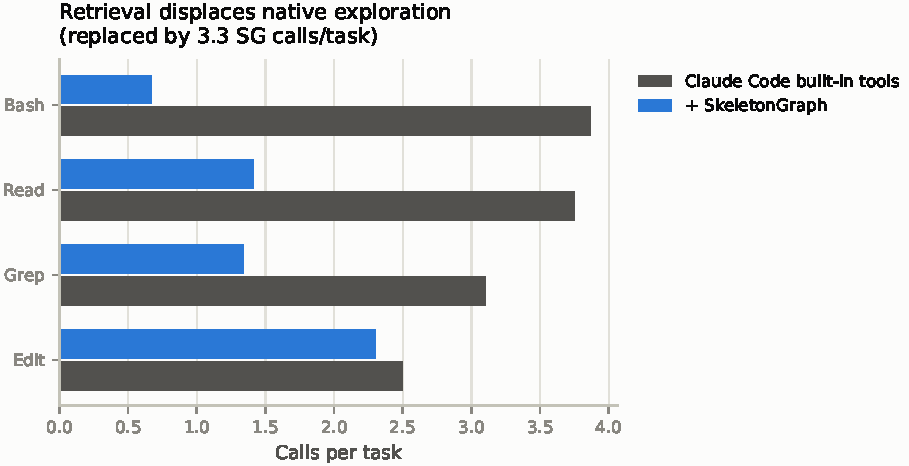
\includegraphics[width=0.80\linewidth]{figures/fig_tool_displacement.pdf}
\caption{Where the turns go. Structural retrieval collapses exploratory
navigation---shell, read, and grep calls all fall sharply---and replaces it with
a small number of targeted retrieval calls. Editing is unchanged, which is
consistent with the residual cost living in implementation rather than search.}
\label{fig:displace}
\end{figure}

\subsection{When breadth is misread as scope}
\label{sec:scope}
Section~\ref{sec:decoupling} reported that \sg{} is more expensive on 60 of 100
tasks, mostly by small margins. Those cases have a consistent cause, and it
follows from the precision measurement: retrieval returns the right region, and
the agent occasionally infers that the whole region needs changing.

The clearest instance is a Django task about form handling. \sg{} retrieved, at
rank one, the base class method responsible for altering database schema---an
entirely correct result, and an architectural hub called by every database
backend. The agent took the hub's centrality as evidence that the fix belonged at
that level, and edited across the base implementation plus the MySQL, Oracle,
PostgreSQL, and PostGIS backends. It spent 38 turns and \$1.32. The baseline,
which found a narrower entry point by text search, made a smaller change in 12
turns and \$0.21. Retrieval was not wrong; it was broad, and breadth was read as
scope.

The same property produces the wins. On an Astropy coordinate-transformation
task, the baseline spent 50 turns and \$1.84 searching for the relevant modules;
\sg{} returned them immediately and the task finished in 14 turns and \$0.43.
Handing over a region is decisive when the agent would otherwise not find it, and
counterproductive when the agent would have found something tighter on its own.

This asymmetry---modest losses on tasks that were already easy to localize, large
wins on tasks that were not---is the tail profile of Table~\ref{tab:tail} restated
at the level of individual runs, and it is why the average and the median
disagree.

\subsection{Four attempts to beat the bound, and why each failed}
\label{sec:interventions}
Section~\ref{sec:floor} predicts that payload shaping has bounded leverage and
that $T$ is not a retrieval variable. We tested that prediction directly, with
four interventions spanning the space. All four are reported; none succeeded.
Their failure modes are individually informative and jointly diagnostic.

\paragraph{(A) Give more, and forbid the alternative.}
We inlined function bodies into search results and disallowed native text search,
forcing retrieval to be the sole path to code. \emph{Prediction:} pushes the
payload above $c^{*}$ and removes the agent's recovery route. \emph{Outcome:}
solve rate fell. Removing the recovery route converts a retrieval miss from a
recoverable detour into an unrecoverable failure, and the inlined bodies were
billed on every subsequent turn.

\paragraph{(B) Remove the need to re-read.}
Returned bodies originally lacked per-line line numbers, so an agent that wanted
to construct an exact edit re-read the file to obtain them. We measured this:
81\% of all re-reads were of material already returned. Adding line numbers
removed the need. \emph{Prediction:} a clean win --- same information, fewer
tokens. \emph{Outcome:} cost fell, and solve rate fell with it --- five losses
against zero gains across 44 paired tasks. Transcripts explain why: the re-read
was not only fetching line numbers, it was the step during which the agent
paused, looked at surrounding code, and then ran the failing test. Removing the
mechanical need removed the incidental behavior. The agent edited and submitted
without executing anything.

This is the most instructive of the four. The "waste" we identified was real, and
eliminating it was still harmful, because the wasteful action was load-bearing for
an unrelated and more valuable behavior. Efficiency interventions on agent
trajectories cannot be validated on the metric they target.

\paragraph{(C) Restore verification explicitly.}
If the verification loop was what (B) destroyed, mandate it: instruct the agent
to reproduce the failure, edit, and re-run before submitting. \emph{Prediction:}
recovers (B)'s losses while keeping its savings. \emph{Outcome:} substantially
worse --- input tokens rose 90\% with no solves recovered. The instruction
converted a calibrated behavior into an unconditional one: the agent ran test
sweeps on tasks that did not need them, and the phrase "confirm nothing else
broke" induced defensive edits far beyond the bug. Verification was already
happening at roughly the right rate; making it mandatory removed the model's
judgment about \emph{when}.

\paragraph{(D) Give only pointers.}
The converse of (A): return only file, symbol and line range --- never bodies ---
and let the agent read what it decides it needs with its own tools.
\emph{Prediction:} pushes below $c^{*}$; the agent recovers the difference, and
tokens relocate rather than disappear. \emph{Outcome:} as predicted. On narrow,
well-scoped tasks the leaner payload was competitive, but on broad tasks the
agent made a small number of retrieval calls, then reverted to extended native
navigation --- and total cost rose. Withholding bodies does not save the tokens;
it moves them from a targeted retrieval call into a longer sequence of untargeted
reads, while adding turns.

\paragraph{(E) Route each task to whichever system suits it.}
The four above shape \emph{what} retrieval returns. A fifth option is to decide
\emph{whether} to retrieve at all: given the crossover in Table~\ref{tab:decile},
send cheap tasks to the built-in tools and expensive ones to \sg{}. This is the
obvious product response, so we measured its ceiling before building it.

An oracle allowed to see both outcomes and pick the cheaper per task spends
\$31.80 against \$37.07 for always using \sg{}---a 14.2\% gain, and that is an
upper bound no implementable rule can exceed. It comes with a defect that rules it
out on its own terms: the oracle's solve rate is 72/100, \emph{below} both always-
\sg{} (75) and never-\sg{} (74). Cheap runs are frequently cheap because the agent
gave up early, so selecting for low cost selects for failure.

Implementable rules do far worse. No feature available before the run separates
the cases: whether the issue names the target file differs by 5 percentage points
between \sg{}'s wins and losses (70\% versus 65\%), issue length by 4\%. Signals
from \sg{}'s own first search are no better---it locates the gold file in 95\% of
its wins and 88\% of its losses. Every threshold rule we simulated on these
signals was worse than simply always retrieving.

The reason is structural, and it is the same wall from a new direction:
\sg{}'s retrieval is \emph{equally good} on cheap and expensive tasks. Expensive
tasks are not ones where retrieval fails; they are ones where the change is
larger---1.54 gold files on average against 1.10, and 23.3 baseline steps against
5.7. Difficulty lives in implementation and validation, so no retrieval-time
signal can forecast it. Predicting cost from retrieval state is a category error.

\paragraph{What the five together show.}
The interventions move in every available direction. (A) and (C) add; (B) and (D)
subtract; (E) declines to act at all on some tasks. Every one degraded cost or
correctness, and the one with a favourable ceiling reaches it by selecting
failures. That is the signature of an optimum, not of insufficient tuning.

Taken with the measurements, this is the evidence for a genuine ceiling rather
than an unexploited opportunity. Four independent observations point at it:

\begin{enumerate}
\item Retrieval accuracy is already near its practical maximum---83.6\% first-search
file recall, ~80\% function identification---and the median task is no cheaper.
Whatever remains is not waiting on better ranking.
\item The agent's peak context is unchanged (44.1k versus 44.9k tokens), so the
term that would need to move in Equation~\eqref{eq:decomp} does not move.
\item \sg{}'s own responses become roughly 70\% of the tokens it carries forward.
It substitutes for the reads it prevents rather than eliminating them.
\item Both directions of payload shaping, and task routing on top, fail.
\end{enumerate}

We state the implication plainly, because it is easy to lose in a results table:
\textbf{beyond a certain point, cost stops responding to retrieval quality at
all.} An agent takes what the task requires regardless of who supplies it, holds
it for the rest of the run, and spends the remainder of its budget implementing
and validating. A retrieval layer buys the localization prefix and nothing after
it---and on tasks where that prefix was already short, it is a net cost.

\subsection{The ceiling belongs to the paradigm, not to our implementation}
\label{sec:ceiling}
A natural objection is that our structural retriever is simply not good enough,
and that a better lexical index, a stronger code embedder, or a richer graph
would close the gap. We can address this directly, because \sg{}-Fusion is not
one paradigm but three operating simultaneously: lexical (BM25), semantic (a
code-specialized dense encoder), and topological (the call graph). If any of the
three could infer which code is responsible for a described symptom, removing the
symbol names from the issue text should not much matter.

We test this by crossing two factors: whether the model has memorized the
repository (the standard benchmark versus a decontaminated one), and whether the
issue text still contains location cues (the original text versus a
prose-stripped variant with tracebacks and code blocks removed).
Figure~\ref{fig:ceiling} shows the result. First-search recall falls from 86\% to
44\% as the cues are withdrawn---and the lexical baseline falls with it, from
66\% to 39\%. The two curves converge: in the prose-only condition on the
memorized benchmark, retrieval augmented with all three paradigms is
\emph{indistinguishable} from built-in lexical search ($-0.006$ recall).

\begin{figure}[t]
\centering
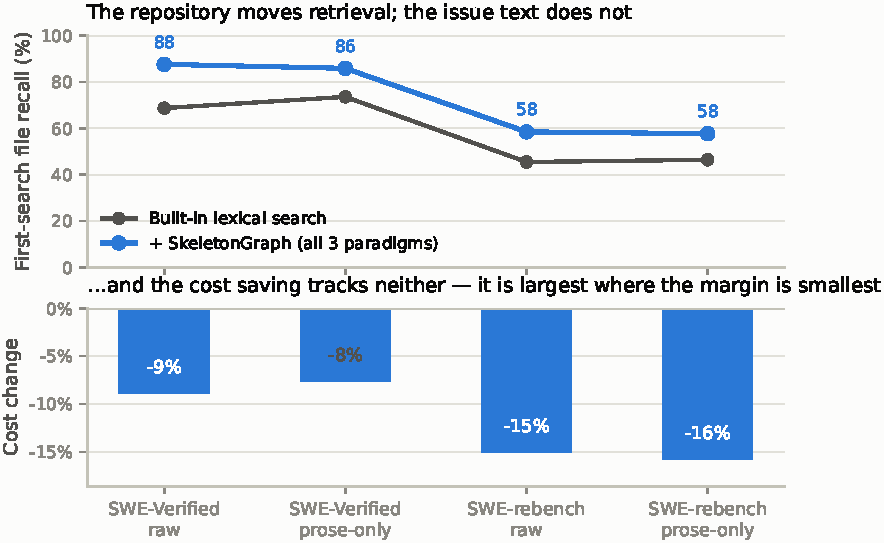
\includegraphics[width=\linewidth]{figures/fig_ceiling.pdf}
\caption{\textbf{Top:} first-search file recall as location cues are removed
(left to right). The advantage of combining lexical, semantic, and topological
retrieval collapses; the baseline declines in parallel, so the limit is a
property of the category rather than of one implementation. \textbf{Bottom:} the
cost saving persists in every condition---including the one where retrieval
quality is identical to the baseline. Retrieval quality is therefore not the
mechanism producing the saving. SWE-Verified columns are restricted to the same
15 tasks as the prose run so that the raw and prose conditions are paired.}
\label{fig:ceiling}
\end{figure}

Two conclusions follow, and they pull in opposite directions. The first is
negative: no combination of non-LLM retrieval paradigms available to us performs
the inference from symptom to responsible code. That inference is causal---it
requires knowing what code \emph{does} when it runs, not what it resembles---and
similarity matching, whether lexical, dense, or topological, does not supply it.
The second is positive, and is the more useful finding: \textbf{the cost saving
survives the collapse of the retrieval advantage.} In the prose-only condition
where recall is identical to the baseline, cost still falls by 21\%. Whatever
\sg{} is doing to reduce cost, it is not out-retrieving the baseline; it is
bounding how far the agent wanders before it commits.

\section{Threats to Validity}
\label{sec:threats}

\paragraph{Contamination.}
Our no-retrieval control establishes that SWE-bench Verified is
memorization-saturated in our setting. We therefore treat solve rate as a
tie-detection instrument, not a ranking signal. We additionally built a
decontaminated replication path against a continuously-updated benchmark drawn
from thousands of Python repositories with tasks postdating model cutoffs. On
that decontaminated set (15 paired tasks, test-execution verified) the direction
of every effect is preserved: cost $-26.4\%$, turns $-35.6\%$, solve rate
10/15 versus 9/15---statistically indistinguishable, as on the contaminated
benchmark. The decontaminated replication therefore does not overturn any claim
in this paper; it reproduces them on repositories the model has not memorized.

\paragraph{Answer leakage through web tools.}
In one trace the agent used its web tools to fetch the upstream pull request
corresponding to the benchmark task---that is, the reference patch. This is
available to any web-enabled agent and is not specific to any retrieval arm, but
it means solve rates for web-enabled frontier agents on public benchmarks should
be treated with caution, and it is a further argument for decontaminated or
private task sets.

\paragraph{Run-to-run variance.}
Agent trajectories are stochastic; single volatile tasks can move aggregate
percentages by double digits at $n\!\approx\!50$. We report distributions and
paired tests rather than point estimates, and flag outliers explicitly.

\paragraph{Scope.}
Headline results are Python. \sg{} parses ten languages, but we do not claim
performance parity outside Python and do not report multi-language solve rates.

\paragraph{Cost model.}
Cost is imputed from token counts under one provider's published pricing,
applied identically across arms. Absolute dollars are indicative; paired
\emph{ratios} are the meaningful quantity.

\section{Discussion}

\subsection{What this means for building code-context systems}
The design space of Section~\ref{sec:designspace} can now be scored against
measurement rather than intuition. Prompt injection is dominated: a map placed in
the fixed prompt is re-sent every turn, which is why the repository-map system
consumes an order of magnitude more tokens for no solve-rate benefit. Graph query
and structural retrieval both pay per use and land within a factor of 1.5 of each
other. Lexical search remains a genuinely strong baseline at file granularity.
The differences among the pay-per-use designs are small relative to the
difference between all of them and the injection design --- so the first-order
engineering decision is \emph{when} context is delivered, not how cleverly it is
selected.

For a builder, the actionable form of our result is: optimize the delivery
schedule before optimizing the ranking. Ranking improvements act on $\Delta T$
through the localization prefix, which is already short. Delivery-schedule
mistakes act on $\bar{c}$ multiplied by every remaining turn.

\subsection{Why we are not claiming more}
It would be straightforward to report this work as a 15\% cost reduction with
improved retrieval accuracy and leave the distribution out. We think that
framing, which is standard in this category, is the reason the category's claims
do not replicate. A mean is not a promise a user experiences: half of our users'
tasks would see no saving at all. What they would see is that their worst tasks
stop running away --- which is a real benefit, precisely stated, and one we can
defend per-task.

We also decline the solve-rate claim available to us. \sg{} won 75 to 74. On a
benchmark where a no-retrieval control scores 36--44\%, that difference is not
evidence of anything, and reporting it as a win would be the same error we
criticize.

\section{Conclusion}
We set out to determine what better code retrieval buys an agent. The answer is
narrower than the design intent and than the field's claims, and it is
structural rather than incidental.

Structural retrieval does what it was designed to do: it returns the function to
edit, at a granularity lexical search does not possess, and it collapses
exploratory navigation. But cost in an agent loop accumulates as
$\sum_t c_t$, and retrieval moves only the localization prefix of $T$ while
leaving $\bar{c}$ unchanged --- because the agent takes what it needs regardless
of who hands it over, and everything taken early is re-sent for the rest of the
trajectory. Push the payload below what the task requires and the agent fetches
the remainder itself; push it above and the surplus is billed every turn. Both
directions were tested, and both cost accuracy.

The consequence is a decoupling: an order-of-magnitude improvement in
function-level retrieval yields no change in median cost and no change in solve
rate, while removing 42.5\% of cost at the 95th percentile. Retrieval is an
anti-catastrophe layer. It bounds the worst case; it does not shift the typical
one. Until an agent's own turn count falls --- which is a property of how it
implements and validates, not of how it searches --- context accumulates and cost
grows with it.

We think this is the more useful claim for practitioners and the more honest one
for the field, and we release the harness, frozen task lists, and per-task records
so that it can be checked rather than trusted.

\bibliographystyle{unsrtnat}   % numeric, ordered by first citation
\bibliography{references}

\end{document}
